% Copyright (c) 2014,2016 Casper Ti. Vector
% Public domain.

\chapter{序言} \label{chap:introduction}
随着多处理器、多核技术的迅猛发展,多核处理器(CMP)中的核数也越来越多。核数增加一个显而易见的优点就是可以支持更多的程序并发执行,然而这也导致了存储访问的瓶颈变得尤为突出。由于中央处理器(CPU)的运算速度远远高于其访问内存的速度,为了缓解这个速度差异,通常在CPU与内存之间会设有多级高速缓存(Cache)。在多核处理器中,每个核会有一到二级私有缓存,同时所有核会共享一个底层缓存(LLC)。由于缓存大小有限,并发执行的程序会对这层共享缓存进行竞争,竞争的结果就是每个程序的性能都或多或少受到损失。

目前CPU大多采用基于LRU的缓存替换策略,它对所有的缓存访问,不管来源于哪个核,都“一视同仁”。这就带来了一个问题:一个污染性高的程序会占据大量的缓存空间,从而压缩了其他程序的缓存使用,导致它们的失效率升高,性能下降。长期以来,国内外对这个问题展开了大量的研究工作,但是这个问题并没有得到完美的解决。前人的研究大多依赖于硬件/软件层面上对共享缓存进行划分,通过对缓存插入和替换策略的调优来改善系统效率。然而,它们大多数都需要硬件修改,只是在模拟器上进行模拟实验,但无法应用到真实系统上。

基于硬件的方法主要是在模拟器中进行实现~\parencite{suh2004dynamic,qureshi2006utility,qureshi2007adaptive,hsu2006communist,iyer2004cqos,kim2004fair,rafique2006architectural,xie2009pipp}。然而模拟器存在多方面的不足,比如运行速度较慢、准确度不够等等。通常一个基于模拟器的实验会运行几十亿条指令,这仅仅相当于实际运行的几秒钟。一个程序的结构和行为的复杂性无法在这么短的执行时间里体现出来。所以我们认为对于一个缓存优化方案,必须要经过长时间的执行才能证明其有效性。

基于软件的方法主要是通过页面着色技术(Page Coloring)。它通过操作系统对页面映射进行控制,从而完成对缓存占用的控制。页面着色技术发明时,主流处理器对于地址到缓存块的映射还是采用Round-robin的方式,所以可以通过操作系统控制页面地址来限制缓存的占用,该技术可以在真实系统中得以实现。然而随着处理器架构的发展,现代处理器纷纷改用哈希算法来处理内存地址到缓存块的映射。所以页面着色技术目前也不再适用了。

缓存调控的另一个关键点是分配的粒度。粗粒度分配技术一般是基于缓存路的划分(Way Partitioning)~\parencite{suh2004dynamic,qureshi2006utility,qureshi2007adaptive,hsu2006communist,iyer2004cqos,kim2004fair,rafique2006architectural,xie2009pipp}。一个路往往含有多个缓存块(Block),划分的时候不能把一个路切开分给两个不同的线程,并且由于体系结构的限制,路的个数不能无限制增加。所以基于路的缓存划分涉及的硬件改动较小,但是粒度较粗。另外一些研究提出了细粒度划分技术~\parencite{sanchez2011vantage,manikantan2012probabilistic,chang2014cooperative}。虽然细粒度划分提供了更强的可扩展性和灵活性,但是需要更加复杂的设计和更多的硬件改动。考虑到设计的简洁性,大部分研究还是采用了粗粒度的路划分技术。正如前文所说,路划分技术下分配的最小单位是一个路,而往往一个路会包含成百上千个缓存块。在核数/线程数增加的情况下,它的效率就会下降,因为最优的划分方案很可能会切在一个路的中间。极端情况下当核数/线程数等于总路数,每个线程有且只能有一个路的缓存分配,这就彻底失去了分配的灵活性。一些研究试图在保留路分配的基础上,细化分配粒度。Probabilistic Shared-Cache Management(PriSM)通过精确控制淘汰(Eviction)概率来把粒度变得更细~\parencite{manikantan2012probabilistic}。Cooperative Cache Partitioning(CCP)通过时域共享,在不同的时间片中切换不同的分配方案,从来提高分配的灵活性~\parencite{chang2014cooperative}。不过,这些研究都或多或少地涉及硬件改动,所以只能在模拟器中进行实验,而暂时无法应用到实际系统中。

在本文中,我们提出了CAPS(Cache Allocation with Partial Sharing),一个基于部分共享的缓存分配优化框架。CAPS在真实系统上实现了细粒度的缓存分配,是一个纯软件的框架。CAPS依赖于英特尔高速缓存分配技术(CAT)。CAT是英特尔最近才在服务器处理器中全线引入的功能,它首次在商业处理器上实现了对高速缓存的管理。CAT也是基于路的划分,所以本身是一个粗粒度的分配技术。CAT技术中可分配的路数非常有限,在最高端的处理器上也只有20个路可供分配,每个路包含数个MB的缓存空间。为此,我们提出了通过空间共享的方式来细化分配粒度,并且空间部分共享分配,换句话说分配之间部分重叠,也是CAT技术所允许的。通过精确地控制分配以及之间的重叠,我们可以实现一个较细粒度的缓存管理。

我们用一个小例子来说明部分共享如何优于完全共享和不共享的分配。两个SPEC CPU2006的测试程序470.lbm和471.omnetpp分别运行在两个核上,它们共享一个4路高速缓存,每路含有2816KB的缓存资源。我们在真实机器上实验了所有可能的CAT分配方案,然后选择最优的重叠方案和不重叠方案。最优这里指的是IPC(周期指令数)吞吐量的最大化,也就是这两个程序的IPC之和最大。图 \ref{fig:illustration} (a) 展示了这三种方案的分配布局,从上到下分别是:传统的完全共享LLC(full share)、最优的不重叠分配(non-overlapping)和最优的重叠分配(overlapping)。图 \ref{fig:illustration} (b) 比较了这三种方案的IPC吞吐量。不难看出,部分重叠的分配方案比另外两种方案都要更优。完全重叠下两个程序的平均IPC分别为0.347和0.955,不重叠下分别为0.421和0.913, 部分重叠下为0.415和0.968。部分重叠相比于完全重叠,两个程序的IPC都获得提升;相比于不重叠分配,虽然470.lbm的IPC稍微损失了一点,但471.omnetpp得到了很大的提升,所以加总的IPC吞吐量也获得了提升。

\begin{figure}[htbp] 
    \centering
    \begin{subfigure}[b]{0.4\linewidth}
        \centering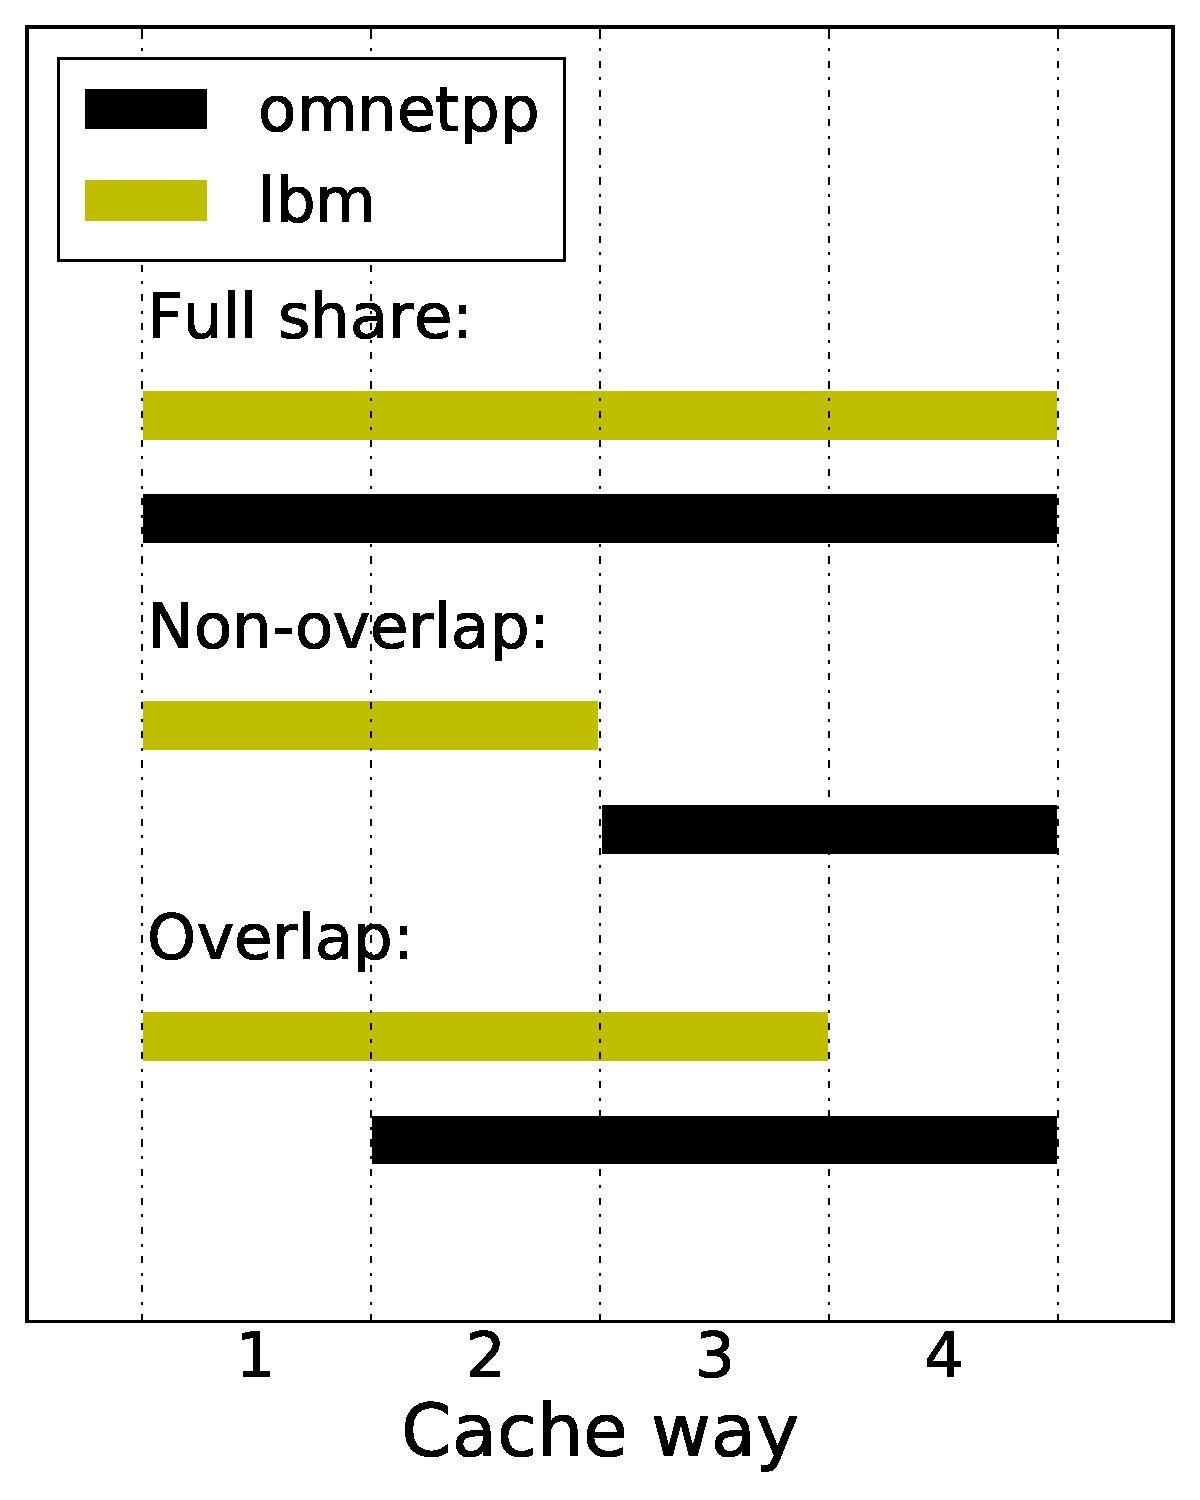
\includegraphics[width=0.9\linewidth]{figures/scheme.pdf}
        \caption{分配布局}
    \end{subfigure}%
    \begin{subfigure}[b]{0.4\linewidth}
        \centering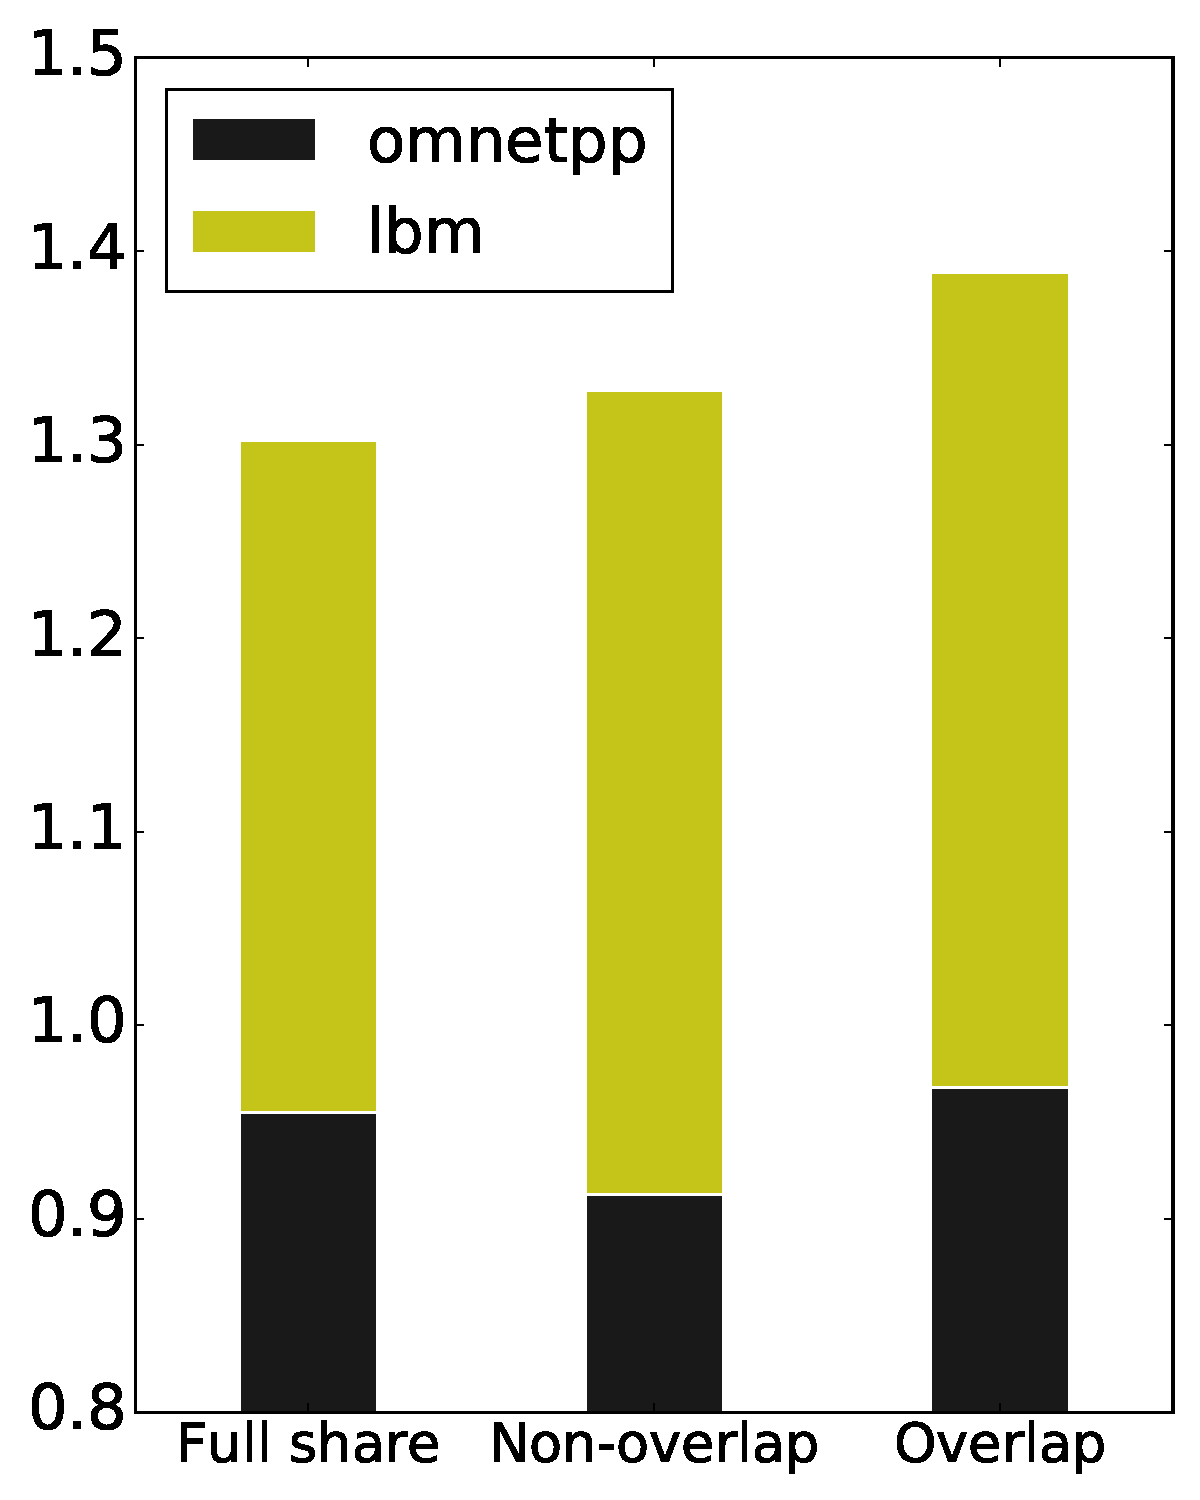
\includegraphics[width=0.9\linewidth]{figures/throughput.pdf}
        \caption{IPC吞吐量}
    \end{subfigure}
    \caption{完全重叠、不重叠和部分重叠方案的比较示例}
    \label{fig:illustration}
\end{figure}

我们更深入的研究表明,随着核数/并发线程数的增加,CAPS生成的部分重叠方案对完全重叠和不重叠划分的优势会愈发明显。CAPS包含两个部分:(1)一个预测模型可以较为准确地预测出在任意重叠CAT分配下(完全共享和不共享划分是两个特例)的并发程序的缓存失效率和IPC;(2)一个优化算法在给定一个优化目标后生成一个优化分配方案。借助于英特尔CAT技术,我们在真机上实现了CAPS并在实际系统中进行了实验评估。在评估实验中,我们把每个并发的程序都运行完毕,同时一些性能指标通过硬件性能计数器(Performance Counter)和高速缓存监控技术(CMT)来收集和记录。CAPS具有高度的灵活性,可以支持很多优化目标和策略。我们在CAPS上实现了5种策略分别锚定5个优化指标:(1)平均每1000条指令缓存失效数(Average MPKI);(2)IPC吞吐量(Throughput);(3)相比于独占缓存,每个程序平均的性能损失(Average Slowdown);(4)兼顾公平的性能损失(Fair Slowdown);(5)最大的性能损失(Maximum Slowdown)。实验结果表明,相比于自由竞争,在Average MPKI这个指标上,CAPS平均可以降低16.96\%的失效数,最好情况下可以降低23.1\%;对于Throughput,CAPS平均提升11.11\%,最好情况下提升高达31.3\%;对于Average Slowdown,CAPS在平均程度上可以减小性能下降8.16\%,最优情况下达到11.18\%;对于Fair Slowdown,平均可以被减小8.17\%,最好情况13.2\%;对于Maximum Slowdown,平均可以提升23.24\%,最好情况下高达33.42\%。

本文提出的CAPS缓存分配优化框架的主要特点和优势有以下几点:

\begin{itemize}
    \item 在细粒度上实现缓存分配。通过精确地控制分配重叠,CAPS突破了路划分技术的分配粒度限制,实现了细粒度的控制,同时也没有带来额外开销。细粒度分配可以带来更好的优化效果。
    \item 支持多种优化策略。过往的研究对于不同的优化目标需要制定不同的策略,而在CAPS中,只需要简单地适配优化函数,就可以实现一个新的策略。这大大增强了优化的灵活性。
    \item 具有良好的可扩展性。随着线程数/核数的增加,可扩展性对于一个优化框架来说格外重要。过去的解决方案多是针对双核/双线程的情景,对于如今动辄十几个核的处理器就会力不从心。而CAPS对于核数少与多的情况都提供了良好的支持。
    \item 可以在真实系统中实现。CAPS是一个纯软件的框架,通过CAT技术得以在真实系统上实现。相比于模拟器,我们在真机上可以进行更加充分的实验。同时,CAPS也更容易被应用到实际生产环境中。
\end{itemize}

据我们所知,CAPS是国内外第一个基于缓存分配技术在真实系统上实现的普适性缓存优化框架,它开创性地利用部分共享缓存空间来增强优化效果。本文的后续部分如下安排:

在第\ref{chap:related}章中,我们介绍了有关高速缓存的重要概念,CAT技术的背景知识,以及国内外相关工作的研究进展。

在第\ref{chap:design}章中,我们将介绍CAPS框架的设计与实现。对于其中最重要的两个模块,预测和分配,我们将分别详细阐述。对于CAPS的性能预测模型,我们探讨了该预测方法的基本原理,并给出算法设计。对于CAPS的优化算法,我们阐述了该算法如何在给定条件下生成一个优化算法,并给出算法伪代码。同时我们会对CAPS中实现的5个优化策略进行进一步分析。

在第\ref{chap:evaluation}章中,我们通过大量的实验对CAPS进行全方位的评估。评估先从宏观角度给出综合性评估分析,再从微观角度对个别实验样本进行细致分析。

最后,我们在第\ref{chap:conclusion}章中,总结了全文的工作成果,并提出未来的研究方向。